
% 
% topic Template for ME3023 - Measurements in Mechanincal Systems - Tennessee Technological University
%
% Spring 2020 - Summer 2020
% Tristan Hill, May 31, 2020
% Module 3 - Calibration
% Topic 1 - Accuracy and Precesion   ->  (4th Topic)
%

%\documentclass{beamer}                         % for presentation (has nav buttons at bottom)
\documentclass[handout]{beamer}  % for handout 
\usepackage{beamerthemesplit}
\usepackage{amsmath}
\usepackage{listings}
\usepackage{multicol}
\usepackage{framed}

\usepackage{soul}

%\usepackage{lrbox}

\beamertemplateballitem

\definecolor{TTUpurple}{rgb}{0.3098, 0.1607, 0.5176} % TTU Purple (primary)
\definecolor{TTUgold}{rgb}{1.0000, 0.8666, 0.0000} % TTU Gold (primary)

\setbeamercolor{palette primary}{bg=TTUpurple,fg=TTUgold}
\setbeamercolor{palette secondary}{bg=black,fg=TTUgold}
\setbeamercolor{palette tertiary}{bg=black,fg=TTUpurple}
\setbeamercolor{palette quaternary}{bg=TTUgold,fg=black}
\setbeamercolor{structure}{fg=TTUpurple} % itemize, enumerate, etc
\setbeamercolor{section in toc}{fg=TTUpurple} % TOC sections

% custom colors 
\definecolor{mygray}{rgb}{.6, .6, .6}
\definecolor{mypurple}{rgb}{0.6,0.1961,0.8}
\definecolor{mybrown}{rgb}{0.5451,0.2706,0.0745}
\definecolor{mygreen}{rgb}{0, .39, 0}
\definecolor{mypink}{rgb}{0.9960, 0, 0.9960}

% color commands
\newcommand{\R}{\color{red}}
\newcommand{\B}{\color{blue}}
\newcommand{\BR}{\color{mybrown}}
\newcommand{\K}{\color{black}}
\newcommand{\G}{\color{mygreen}}
\newcommand{\PR}{\color{mypurple}}
\newcommand{\PN}{\color{mypink}}

\newcommand{\Lagr}{\mathcal{L}} % lagrangian

\newcommand{\hspcu}{\underline{\hspace{25mm}}} % large horizontal space w underline

\newcommand{\vspccc}{\vspace{6mm}\\} % large vertical space
\newcommand{\vspcc}{\vspace{4mm}\\}   % medium vertical space
\newcommand{\vspc}{\vspace{2mm}\\}     % small vertical space

\newcommand{\hspcccc}{\hspace{10mm}} % large horizontal space
\newcommand{\hspccc}{\hspace{6mm}} % large horizontal space
\newcommand{\hspcc}{\hspace{4mm}}   % medium horizontal space
\newcommand{\hspc}{\hspace{2mm}}     % small horizontal space


\author{ME3023 - Measurements in Mechanical Systems} % original formatting from Mike Renfro, September 21, 2004

\newcommand{\MNUM}{3\hspace{2mm}} % Module number
\newcommand{\TNUM}{3\hspace{2mm}} % Topic number  ->  (4th Topic)
\newcommand{\moduletitle}{Calibration }
\newcommand{\topictitle}{Linear Regression} 

\newcommand{\sectiontitleI}{Motivation - Functional Relationship}
\newcommand{\sectiontitleII}{Least Squares Regression}
\newcommand{\sectiontitleIII}{Using Software Packages}
\newcommand{\sectiontitleIV}{Example: IR Sensor Calibration}


\newsavebox{\mybox}

\title{Lecture Module - \moduletitle}

\date{Mechanical Engineering\vspc Tennessee Technological University}

\begin{document}

\lstset{language=MATLAB,basicstyle=\ttfamily\small,showstringspaces=false}

\frame{\titlepage \center\begin{framed}\Large \textbf{Topic \TNUM - \topictitle}\end{framed} \vspace{5mm}}

% Section 0: Outline
\frame{

\large \textbf{Topic \TNUM - \topictitle} \vspace{3mm}\\

\begin{itemize}
	\item \sectiontitleI		\vspc % Section I
	\item \sectiontitleII 	\vspc % Section II
	\item \sectiontitleIII 	\vspc %Section III
	\item \sectiontitleIV 	\vspc %Section IV
\end{itemize}

}

% Section I:
\section{\sectiontitleI}

\frame{
\frametitle{\sectiontitleI}

A measured variable is often a function of one or more independent variables that are controlled during the measurement. ... This is a common procedure used to document the relationship between the measured variable and an independent process variable. ... \vspccc

We can use {\hspcu} analysis to establish a \hspcu between the \hspcu \hspcu and the \hspcu \hspcu. This discussion pertains directly to \hspcu curve fits.\vspcc

Other functions such as \hspcu and \hspcu fits can also be used.

\vspace{10mm}
{\tiny Text: T.HIll, \underline{Theory and Design of Mechanical Measurements, 5th Edition} }

}

\frame{
\frametitle{\sectiontitleII}


		Consider the graphs below. This is a calibration curve.
 		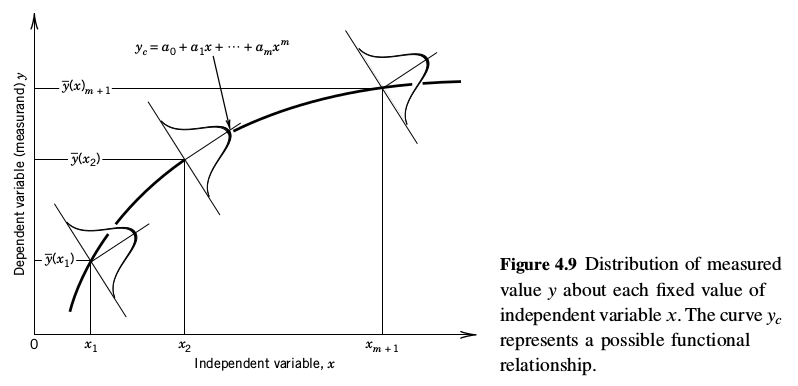
\includegraphics[scale=0.40]{lecture4_fig1.png}
 		{\tiny Image: \underline{Theory and Design of Mechanical Measurements, 5th Edition} }


}


% Section II:
\section{\sectiontitleII}

\frame{
\frametitle{\sectiontitleIII}

	\begin{itemize}
		
		\item We are trying to find a \hspcu \hspcu for the data. \vspc
		\scalebox{1.0}{$y_c(x)=$} \vspc

		\item This is done by \hspcu the quantity below.\vspc
		\scalebox{1.0}{$D=\Sigma_{i=1}^N(y_i-y_{ci})^2=\Sigma_{i=1}^N(y_i-a_0+a_1x+a_2x^2+\dots+a_mx^m)^2$} \vspc

		\item For a \hspcu curve the coefficients become: \vspcc
		
		\scalebox{1.0}{$a_0=$} \hspc, \scalebox{1.0}{$a_1=$}

	\end{itemize}	

}

% Section III:
\section{\sectiontitleIII}

\frame{
\frametitle{\sectiontitleIII}

 Most spreadsheet and engineering software packages can perform a \hspcu on a
data set. Examples will be shown throughout the course in MATLAB and EXCEL.\vspcc
	\begin{itemize}
	
	\item 
	\item 
	\item 
	\item 
	
	
	
	\end{itemize}

}


% Section IV:
\section{\sectiontitleIV}

\frame{
\frametitle{Sample Calibration Data}

\begin{tabular}{|c|c|c|}\hline
Sample \# & Known Distance $x_i (m)$ & Measured Voltage $y_i (V)$ \\ \hline \hline
1&&\\ \hline
2&&\\ \hline
3&&\\ \hline
4&&\\ \hline
5&&\\ \hline
\end{tabular}

\vspace{5mm}
Linear Least Squares Regression Coefficients: \\
\scalebox{1}{$a_0=\hspace{20mm},\hspcc a_1=$} 

Functional Relationship: \\
\scalebox{1}{$y=$}

}

\frame[containsverbatim]{
\frametitle{ Linear Regression in MATLAB - Manual}

\begin{lrbox}{\mybox}
\begin{lstlisting}
clear variables;close all;clc

x=[9 12 15 18 21];
y=[1.17 0.89 0.72 0.61 0.53];
n=length(x);

% perform Linear Least Squares Regression 
a0=(sum(x)*sum(x.*y)-sum(x.^2)*sum(y))/(sum(x)^2-n*sum(x.^2));
a1=(sum(x)*sum(y)-n*sum(x.*y))/(sum(x)^2-n*sum(x.^2));

x_f=5.0:1.0:25;
y_f=a1*x_f+a0;

% generate 1st order curve fit with polyfit()
P1=polyfit(x,y,1);

x_f1=5.0:1.0:25;
y_f1=P1(1)*x_f1+P1(2);
\end{lstlisting}
\end{lrbox}

%\scalebox{0.8}{\usebox{\mybox}}

}

\frame[containsverbatim]{
\frametitle{ Linear Regression in MATLAB - Manual}

\begin{lrbox}{\mybox}
\begin{lstlisting}
figure(1);hold on

plot(x,y,'r*')
plot(x_f,y_f,'m-')
plot(x_f1,y_f1,'b--')

title('First Order Calibration')
xlabel('Known Distance (m)')
ylabel('Measured Voltage (V)')
legend('Raw Data','Linear Fit (T.Hill)','Linear Fit (polyfit)')
grid on
\end{lstlisting}
\end{lrbox}

%\scalebox{0.8}{\usebox{\mybox}}

}

\frame{
\frametitle{ First Order Calibration Curve}

		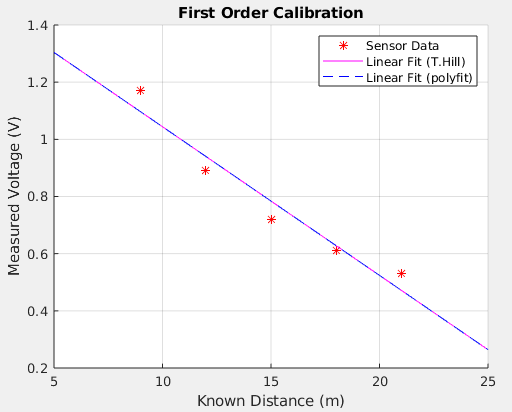
\includegraphics[scale=0.4]{calibration_fig2.png} 
 		{\tiny Images: T.Hill }

}

\frame{
\frametitle{ Fourth Order Calibration Curve}
		
		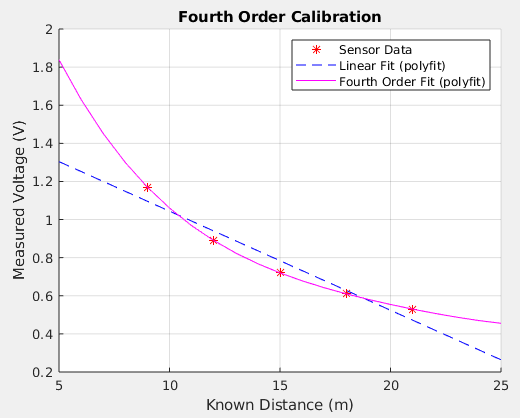
\includegraphics[scale=0.29]{calibration_fig1.png} \hspc  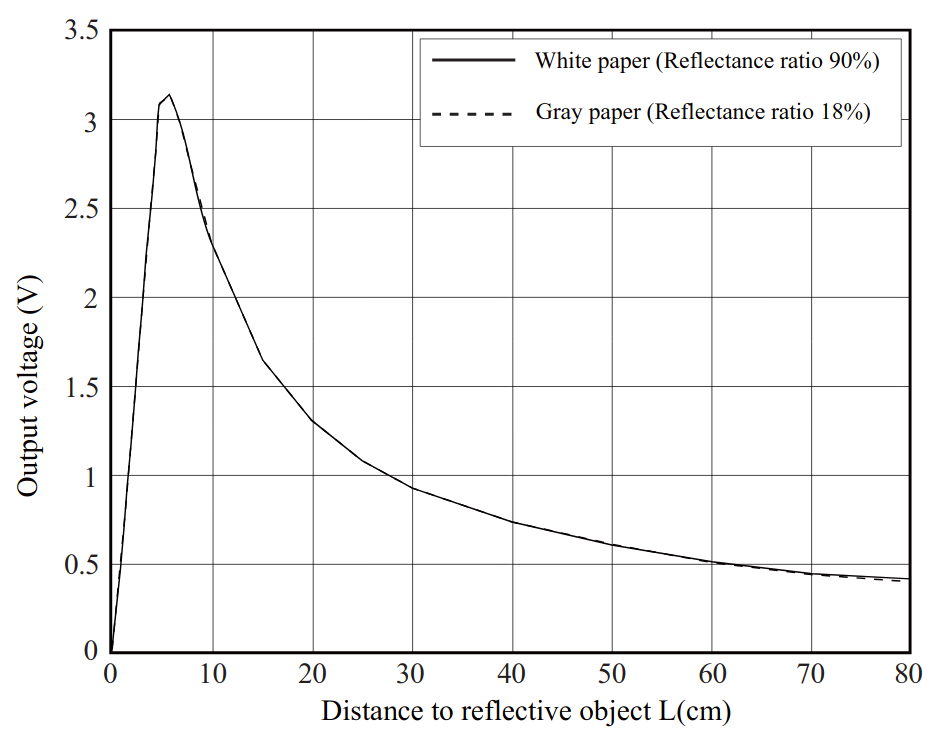
\includegraphics[scale=0.15]{sharp_calibration_fig1.png}\vspc
 		{\tiny Images: T.Hill, Sharp }

}

\end{document}

